Artificial intelligence has become central in corporate disclosure, but outsiders cannot easily verify whether that language reflects implementation. AI-related investments can affect innovation and growth (Babina et al., 2024; Cao et al., 2024). Prior evidence shows that investors treat AI narratives in mandatory filings as informative rather than generic boilerplate (Basnet et al., 2025). In our data, AI language in annual reports expands faster than contemporaneous AI patenting. Figure~\ref{fig:mismatch_surge} shows the scale of this gap. To capture it, we build PatentMismatch, an indicator that flags AI-talking firm-years in which the language tilts toward vague rather than concrete AI content and the firm patents little in AI relative to its industry that year. PatentMismatch characterizes more than 40\% of AI-talking firm-years in both 2024 and 2025. The post-2022 surge in AI disclosure therefore does not simply mirror a comparable surge in implemented AI capability.

\begin{figure}[H]
\centering
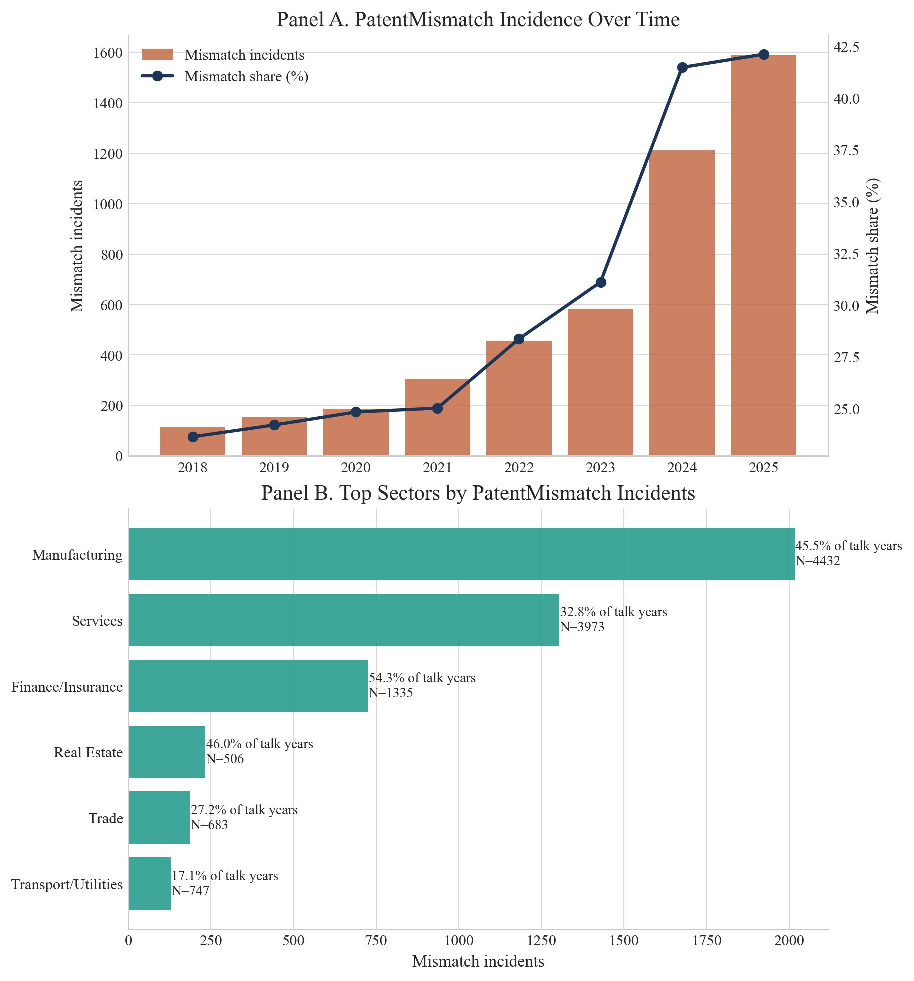
\includegraphics[width=\textwidth]{figures/figure1_main.pdf}
\caption{The rise of low-credibility AI disclosure, 2018--2025}
\label{fig:mismatch_surge}
\begin{minipage}{0.9\textwidth}
\footnotesize
\textit{Note:} This figure plots the share of AI-talking firm-years flagged as PatentMismatch. AI-talking firm-years are firm-years with at least one AI-related sentence in the 10-K filing. Panel A shows the count of flagged firm-years and the mismatch share over time. Panel B shows the mismatch share within the sectors that account for the most AI-talking firm-years.
\end{minipage}
\end{figure}

The credibility problem extends beyond AI. When implementation is costly, salient, and difficult to verify, disclosure can convey information while remaining only loosely tied to realized action. Classic signaling models formalize this logic (Spence, 1973; Seidmann \& Winter, 1997). Adjacent washing literatures document the same problem empirically. Public claims can outrun later observable conduct when investors, regulators, or other stakeholders care about the topic (Delmas \& Burbano, 2011; Kim \& Lyon, 2015; Lyon \& Montgomery, 2015; Baker et al., 2024). AI-related disclosure fits this setting because firms can invoke a valuable technology before outside observers can verify implementation. The central question is whether filing language separates credible AI disclosure from narrative positioning, and whether that distinction predicts realization, organizational response, and market outcomes.

In addition, recent work studies AI communication more directly. The closest published evidence shows that investors respond differently to actionable and speculative AI language in 10-K business descriptions (Basnet et al., 2025). Related work links AI disclosure to later firm outcomes and broader AI narratives to later return patterns (Cao et al., 2024; Bandyopadhyay et al., 2023). Recent working papers compare AI claims with later implementation or capability proxies (Li, 2025; Donelson et al., 2025; Barrios et al., 2025). A remaining gap is an auditable, scalable filing-based framework that links disclosure composition to contemporaneous implementation and later realization.

To fill that gap, we use annual 10-K filings of U.S. public firms from 2016 to 2025. We classify AI-related sentences as actionable, speculative, or irrelevant, aggregate those classifications into firm-year disclosure measures, and use the actionable-to-speculative (AS) ratio together with contemporaneous patent weakness to construct PatentMismatch. The tests first validate PatentMismatch against later AI realization, then examine scrutiny and incentive responses, and finally turn to market outcomes.

The validation evidence begins with later AI realization. PatentMismatch rises sharply after 2022 and becomes common among AI-talking firms. Across alternative construct definitions, the main PatentMismatch measure predicts weaker subsequent AI patent grants. Application-based variants are broader: later AI applications can rise even when near-term patent-grant realization is weak. Among AI-talking firms, mismatch years are followed by lower profitability and higher R\&D intensity, consistent with weaker near-term operating performance and later resource reallocation rather than immediate technological realization.

Disclosure credibility also varies with scrutiny, incentives, and financing windows. Among continuing AI disclosers, disclosure composition becomes more credible after first SEC comment-letter scrutiny, without a comparable decline in AI focus. A public SEC salience event points in the same direction. After the March 18, 2024 AI-washing enforcement actions (SEC, 2024), pre-exposed firms appear to clean up disclosure composition. The March 2024 pattern is best interpreted as salience or acceleration, not as a sharply identified enforcement effect. Inside the firm, low-credibility AI disclosure is more common where CEO equity incentives are stronger. Around first large equity-issuance windows, credibility deteriorates into the financing event and partly unwinds afterward, while AI focus continues to rise. Low-credibility AI disclosure is concentrated where scrutiny, incentives, and financing conditions should matter.

Return evidence is more limited than the validation and organizational-response evidence. Filing-date abnormal returns do not distinguish mismatch from non-mismatch firms, and the broader market block is mixed and benchmark-sensitive. The benchmarked portfolio evidence is strongest in a short-horizon equal-weight post-filing alpha. The corresponding value-weight evidence is weak. Issue-window tests show that the short-run return relation is state-dependent and less negative inside financing windows than outside them. Return tests therefore point to limited and state-dependent pricing of disclosure credibility rather than a broad pricing-anomaly interpretation.

We contribute a filing-based, auditable construct for low-credibility AI disclosure and evidence on when it matters. PatentMismatch predicts weaker subsequent AI patent grants and weaker operating performance, and it is most common where scrutiny, incentives, and financing windows should bear on narrative credibility. Read together, the results describe AI washing as a disclosure-credibility problem that links firms' AI narratives to their later technological and organizational outcomes.

Section 2 places the paper in the disclosure-credibility, washing, and textual-analysis literatures. Section 3 describes the data, the sentence-classification pipeline, the disclosure measures, and the empirical design. Section 4 reports the realization, scrutiny, incentive, financing-window, and market-pricing results. Section 5 discusses what the evidence does and does not establish.
